\pgfmathdeclarefunction{speed}{3}{%
	\pgfmathparse{#3 * ( (1)/(1+exp(4*((#1/2)-x)*#2/#3)) - 1 )}%
}

\newslide{Obstacle Avoidance}{
	\begin{columns}[c]
	\column{0.2\textwidth}
	\begin{tikzpicture}[>=latex',scale=0.4]
	\drawplanexy{-0.3}{-0.3}{-0.3}{6.7}{10}{dashed}{perception}
	
	\drawcube{0}{0}{5}{6.4}{1}{white}{dinamica}{}{};
	\drawcube{0}{1.2}{5}{6.4}{1}{white}{tracking}{}{};
	
	\drawcube{0}{2.4}{5}{6.4}{1}{gray!40}{ostacoli}{}{};
	\drawcube{0}{3.6}{5}{6.4}{1}{white}{altitude}{}{};
	
	\drawcube{0}{4.8}{5}{3}{1.5}{white}{source}{}{};
	\drawcube{0}{6.5}{5}{3}{1.5}{white}{emulatore}{}{};

	\drawplanezy{3.2}{4.8}{5}{4.5}{radar_det}{fill=white,opacity=0.90}{}{};

	\drawcube{3.4}{4.8}{5}{3}{3.2}{white}{alpha}{}{};
	\drawplanexy{-0.3}{-0.3}{5.3}{6.7}{10}{dashed}{action}
	

	\draw [->,line width=1.5] (action_D) -- ++(0,0,2);
	\draw [->,line width=1.5] (perception_D) -- ++(0,0,2);

	\coordinate [at=(radar_det_D), yshift=-5] (arrows_point);
	\draw [->,dashed]  (arrows_point) -- ++(1.5,0,0); 
	\draw [->,dashed]  (arrows_point) -- ++(-1.5,0,0); 
	\end{tikzpicture}
	\vspace{6.5cm}
	\column{0.8\textwidth}
		\begin{block}{}
		
		\begin{tikzpicture}
			\node (immagine) {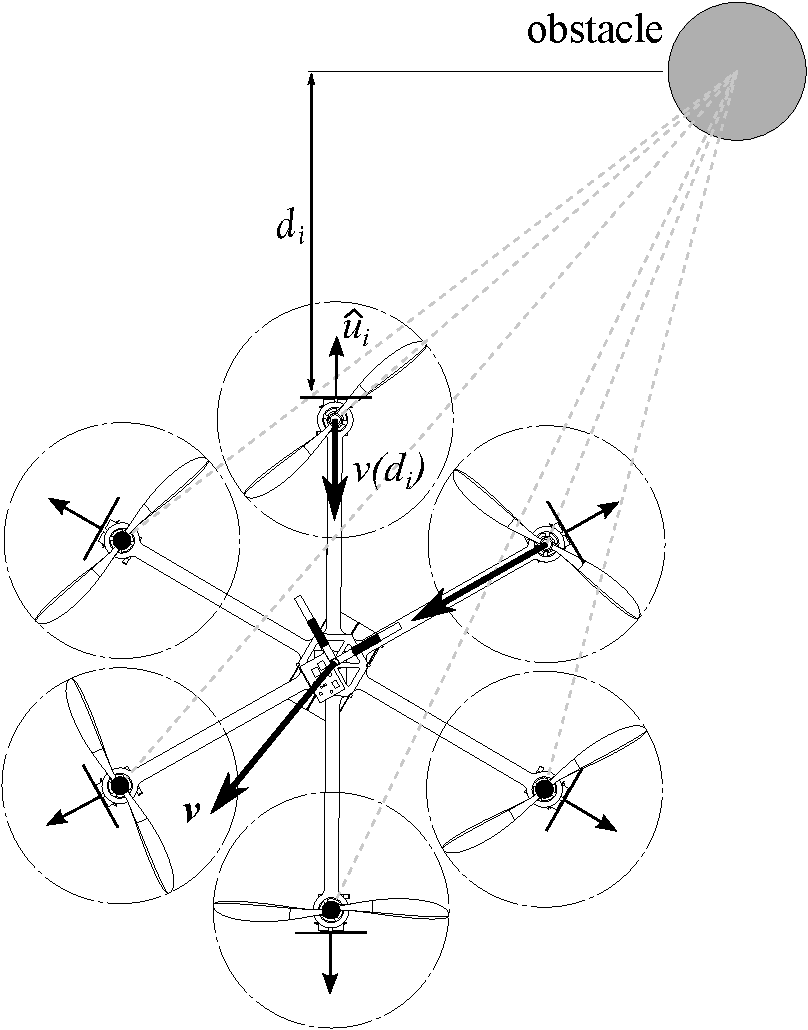
\includegraphics[scale=0.5]{img/obstavoid_dist.pdf}};
			\node [at=(immagine.east), anchor=west, yshift=2.5cm] (velocita) {$
			\mathbf{v} = \mathcal{R}(\phi,\psi,\theta) \sum\limits_{i=1}^6 v(d_i) \left[
				\begin{array}{c} 
					\cos\left((i-1) \dfrac{\pi}{3} \right) \\ 
					-\sin\left((i-1) \dfrac{\pi}{3} \right) \\ 
					0 
				\end{array}
				\right]
			$};
			
			\node [at=(velocita.south), anchor=north, text width=8cm] (grafico) {
			{\small 
				\begin{itemize}
				\item Advantages
				\begin{itemize}
					\item low computation needed
					\item minor constraint on upper layers
					\item fit QFD constraints
				\end{itemize}
				\item Drawbacks
				\begin{itemize}
					\item non--optimal paths
					\item limited reliability
				\end{itemize}
				\end{itemize}
			}
			\vspace{0.75cm}
			Speed function example:
			
			$v(d_i) = p_3 \braces{\dfrac{1}{1+e^{4 \braces{\frac{p_1}{2}-d_i}\frac{p_2}{p_3}}}-1}$
			};
		\end{tikzpicture}
		\end{block}
	\end{columns}
}